%%% LaTeX Template: Article/Thesis/etc. with colored headings and special fonts
%%%
%%% Source: http://www.howtotex.com/
%%% Feel free to distribute this template, but please keep to referal to http://www.howtotex.com/ here.
%%% February 2011
%%%
%%% Modified January 2018 by CDM

%%%  Preamble
\documentclass[11pt,letterpaper]{article}
\usepackage[margin=1.0in]{geometry}
\usepackage[T1]{fontenc}
\usepackage[bitstream-charter]{mathdesign}
\usepackage[latin1]{inputenc}					
\usepackage{amsmath}						
\usepackage{xcolor}
\usepackage{cite}
\usepackage{hyphenat}
\usepackage{graphicx}
\usepackage{float}
\usepackage{subfigure}
\usepackage{sectsty}
\usepackage[compact]{titlesec} 
\usepackage[tablegrid]{vhistory}
\allsectionsfont{\color{accentcolor}\scshape\selectfont}

%%% Definitions
\definecolor{accentcolor}{rgb}{0.0,0.0,0.5} 
\newcommand{\teamname}{Team Friendship}
\newcommand{\productname}{Automated Home Brewing System}
\newcommand{\coursename}{CSE 4316: Senior Design I}
\newcommand{\semester}{Spring 2020}
\newcommand{\docname}{System Requirements Specification}
\newcommand{\department}{Department of Computer Science \& Engineering}
\newcommand{\university}{The University of Texas at Arlington}
\newcommand{\authors}{Luke Brown \\ Marcos Juarez Casillas \\ Ju Young Isa Jung \\ Sujan Dumaru \\ Sunghwa Cho \\ Matthew Francis Schultz}

%%% Headers and footers
\usepackage{fancyhdr}
	\pagestyle{fancy}						% Enabling the custom headers/footers
\usepackage{lastpage}	
	% Header (empty)
	\lhead{}
	\chead{}
	\rhead{}
	% Footer
	\lfoot{\footnotesize \teamname \ - \semester}
	\cfoot{}
	\rfoot{\footnotesize page \thepage\ of \pageref{LastPage}}	% "Page 1 of 2"
	\renewcommand{\headrulewidth}{0.0pt}
	\renewcommand{\footrulewidth}{0.4pt}

%%% Change the abstract environment
\usepackage[runin]{abstract}			% runin option for a run-in title
%\setlength\absleftindent{30pt}			% left margin
%\setlength\absrightindent{30pt}		% right margin
\abslabeldelim{\quad}	
\setlength{\abstitleskip}{-10pt}
\renewcommand{\abstractname}{}
\renewcommand{\abstracttextfont}{\color{accentcolor} \small \slshape}	% slanted text

%%% Start of the document
\begin{document}

%%% Cover sheet
{\centering \huge \color{accentcolor} \sc \textbf{\department \\ \university} \par}
\vspace{0.5 in}
{\centering \huge \color{accentcolor} \sc \textbf{\docname \\ \coursename \\ \semester} \par}
\vspace{0.5 in}
\begin{figure}[h!]
	\centering
   	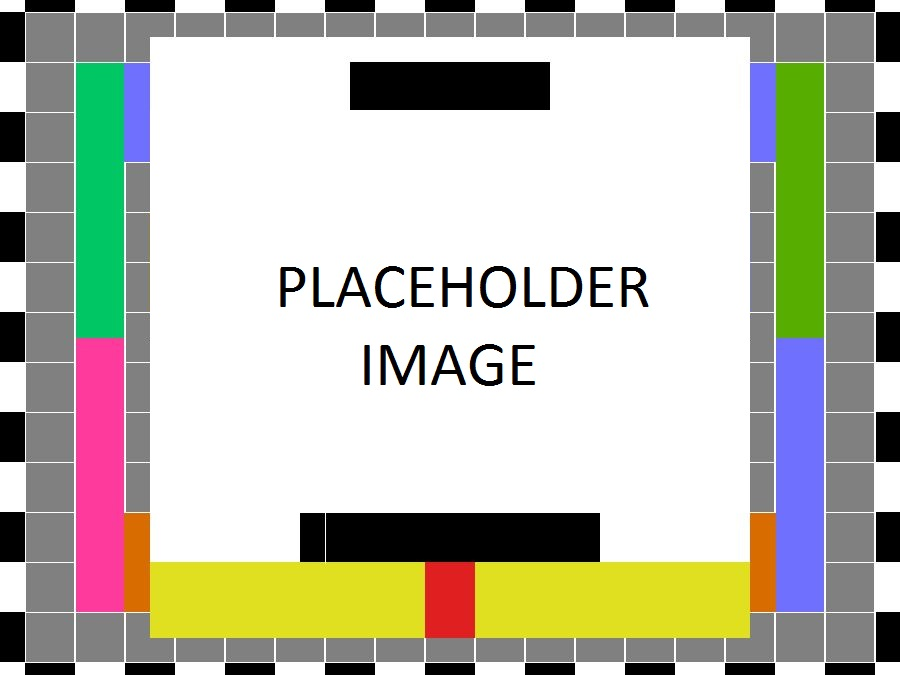
\includegraphics[width=0.60\textwidth]{images/test_image}
\end{figure}
\vspace{0.5 in}
{\centering \huge \color{accentcolor} \sc \textbf{\teamname \\ \productname} \par}
\vspace{0.5 in}
{\centering \large \sc \textbf{\authors} \par}
\newpage


%%% Revision History
\begin{versionhistory}
  	\vhEntry{0.1}{10.01.2015}{GH}{document creation}
  	\vhEntry{0.2}{10.05.2015}{AT|GH}{complete draft}
  	\vhEntry{0.3}{10.12.2015}{AT|GH}{release candidate 1}
  	\vhEntry{1.0}{10.20.2015}{AT|GH|CB}{official release}
  	\vhEntry{1.1}{10.31.2015}{AL}{added customer change requests}
\end{versionhistory}
\newpage

%%% Table of contents
\setcounter{tocdepth}{2}
\tableofcontents
\newpage

%%% List of figures and tables (optional)
\listoffigures
%\listoftables
\newpage

\section{Product Concept}
The "Back Burner Brew" is built with the sole purpose of brewing large batch of beer in the home environment. This product provides home brewers with a low-cost electric home brewing system that allow them to have precise control over the brewing process. The brewing process can be automated with the help of micro-controllers like the ESP32 which is then hosted to a local website or an app interface.

\subsection{Purpose and Use}
ESP32 is a micro-controller that can receive data such as current temperature of the water or mash from the heat sensors located inside the kettles which can be converted to either analog or digital input. The heating coil can be control using the input from the user as per their desired either to increase or to decrease the temperature. The electric pump can also be controlled by the user through micro-controller to regulate the flow of the water in the kettles. The user will be able to communicate with the brewing system through a web interface or app interface.

\subsection{Intended Audience}
The foremost intended audiences for this product would be home brewers or person interested in brewing beer only. Provided that the user manual would be present in the product, any person who wants to brew beer in his local environment can easily use this product. This product is made focusing on how effortless can the brewing process gets simply with the use of micro-controller.

\begin{figure}[H]
	\centering
	\graphicspath{.\images}
	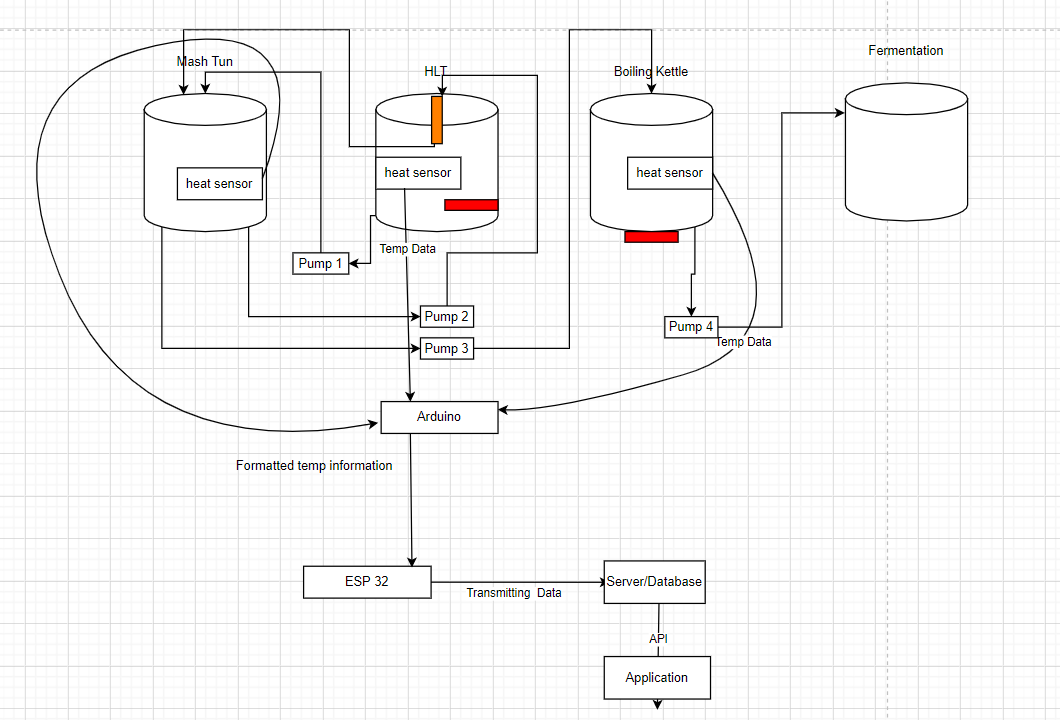
\includegraphics[scale=0.5]{images/sys_overview.PNG}
	\caption{Product Concept}
\end{figure}
\newpage
\section{Product Description}
This section provides a description of your product and defines it's primary features and functions. The purpose is to give the document reader/reviewer enough information about the product to allow them to easily follow the specification of requirements found in the remainder of the document. Your header for this section should introduce the section with a brief statement such as: "This section provides the reader with an overview of X. The primary operational aspects of the product, from the perspective of end users, maintainers and administrators, are defined here. The key features and functions found in the product, as well as critical user interactions and user interfaces are described in detail." Using words, and pictures or graphics where possible, specify the following:

\subsection{Features \& Functions}
What the product does and does not do. Specify in words what it looks like, referring to a conceptual diagram/graphic (Figure X).  Define the principle parts/components of the product. Specify the elements in the diagram/graphic that are part(s) of this product as well as any associated external elements (e.g., the Internet, an external web server, a GPS satellite, etc.)

\subsection{External Inputs \& Outputs}
Describe critical external data flows. What does your product require/expect to receive from end users or external systems (inputs), and what is expected to be created by your product for consumption by end users or external systems (outputs)? In other words, specify here all data/information to flow into and out of your systems. A table works best here, with rows for each critical data element, and columns for name, description and use.

\subsection{Product Interfaces}
Specify what all operational (visible) interfaces look like to your end-user, administrator, maintainer, etc. Show sample/mocked-up screen shots, graphics of buttons, panels, etc. Refer to the critical external inputs and outputs described in the paragraph above.

\newpage
\section{Customer Requirements}
The user should expect to input desired commands, controls, and specific
settings such as temperature and length of time by a easily accessible
touchscreen. The touchscreen will be attached to a Raspberry Pi that will handle
communications between the user and the various sensors and heating elements.
The user can expect that whichever temperature they set for their desired
application, that the temperature will remain constant.

\subsection{Touchscreen Control System}

\subsubsection{Description}
The user needs a way to be able to input commands and specific settings before
starting the beer brewing process. This will be done by attaching a touchscreen
to a Raspberry Pi 4. The Raspberry Pi will then communicate with the automated
brewing system through a webserver that is hosted by the various
microcontrollers that manage various sensors. 

\subsubsection{Source}
This requirement came from Dr. Chris Conly. He requested that our team have a
method by which the user can interface with the automated brewing system and
input various commands, controls, and recipe specific settings.
\subsubsection{Priority}
This feature is of \textbf{Critical} priority. Without this feature the user
would be unable to make the automated brewing system produce the user's desired results. 

\subsection{Programmable HLT Heating Element Temperature Management}
\subsubsection{Description}

The heating element on the HLT will need to maintain the temperature that is set
by the user via the main control touchscreen. The reason for customizable temperature is due to the varying
temperature requirements set by the recipe chose by the user. This temperature control will
managed by an ESP32 microcontroller. The temperature of the vessel will be
monitor by a DS18B20 digital thermometer. The microcontroller will take
continuous readings from the thermometer. When it begins dropping below the
desire temperature the microcontroller will send a signal to a mosfet. When the
mosfet receives that signal it switch states and allow for power to be delivered
to the heating element. Once the desired temperature is reached, the
microcontroller will send another signal to the mosfet. The mosfet will then
turn off, and this would turn off the power to the heating element.

\begin{figure}[H]
	\centering
	\graphicspath{.\images}
	\fbox{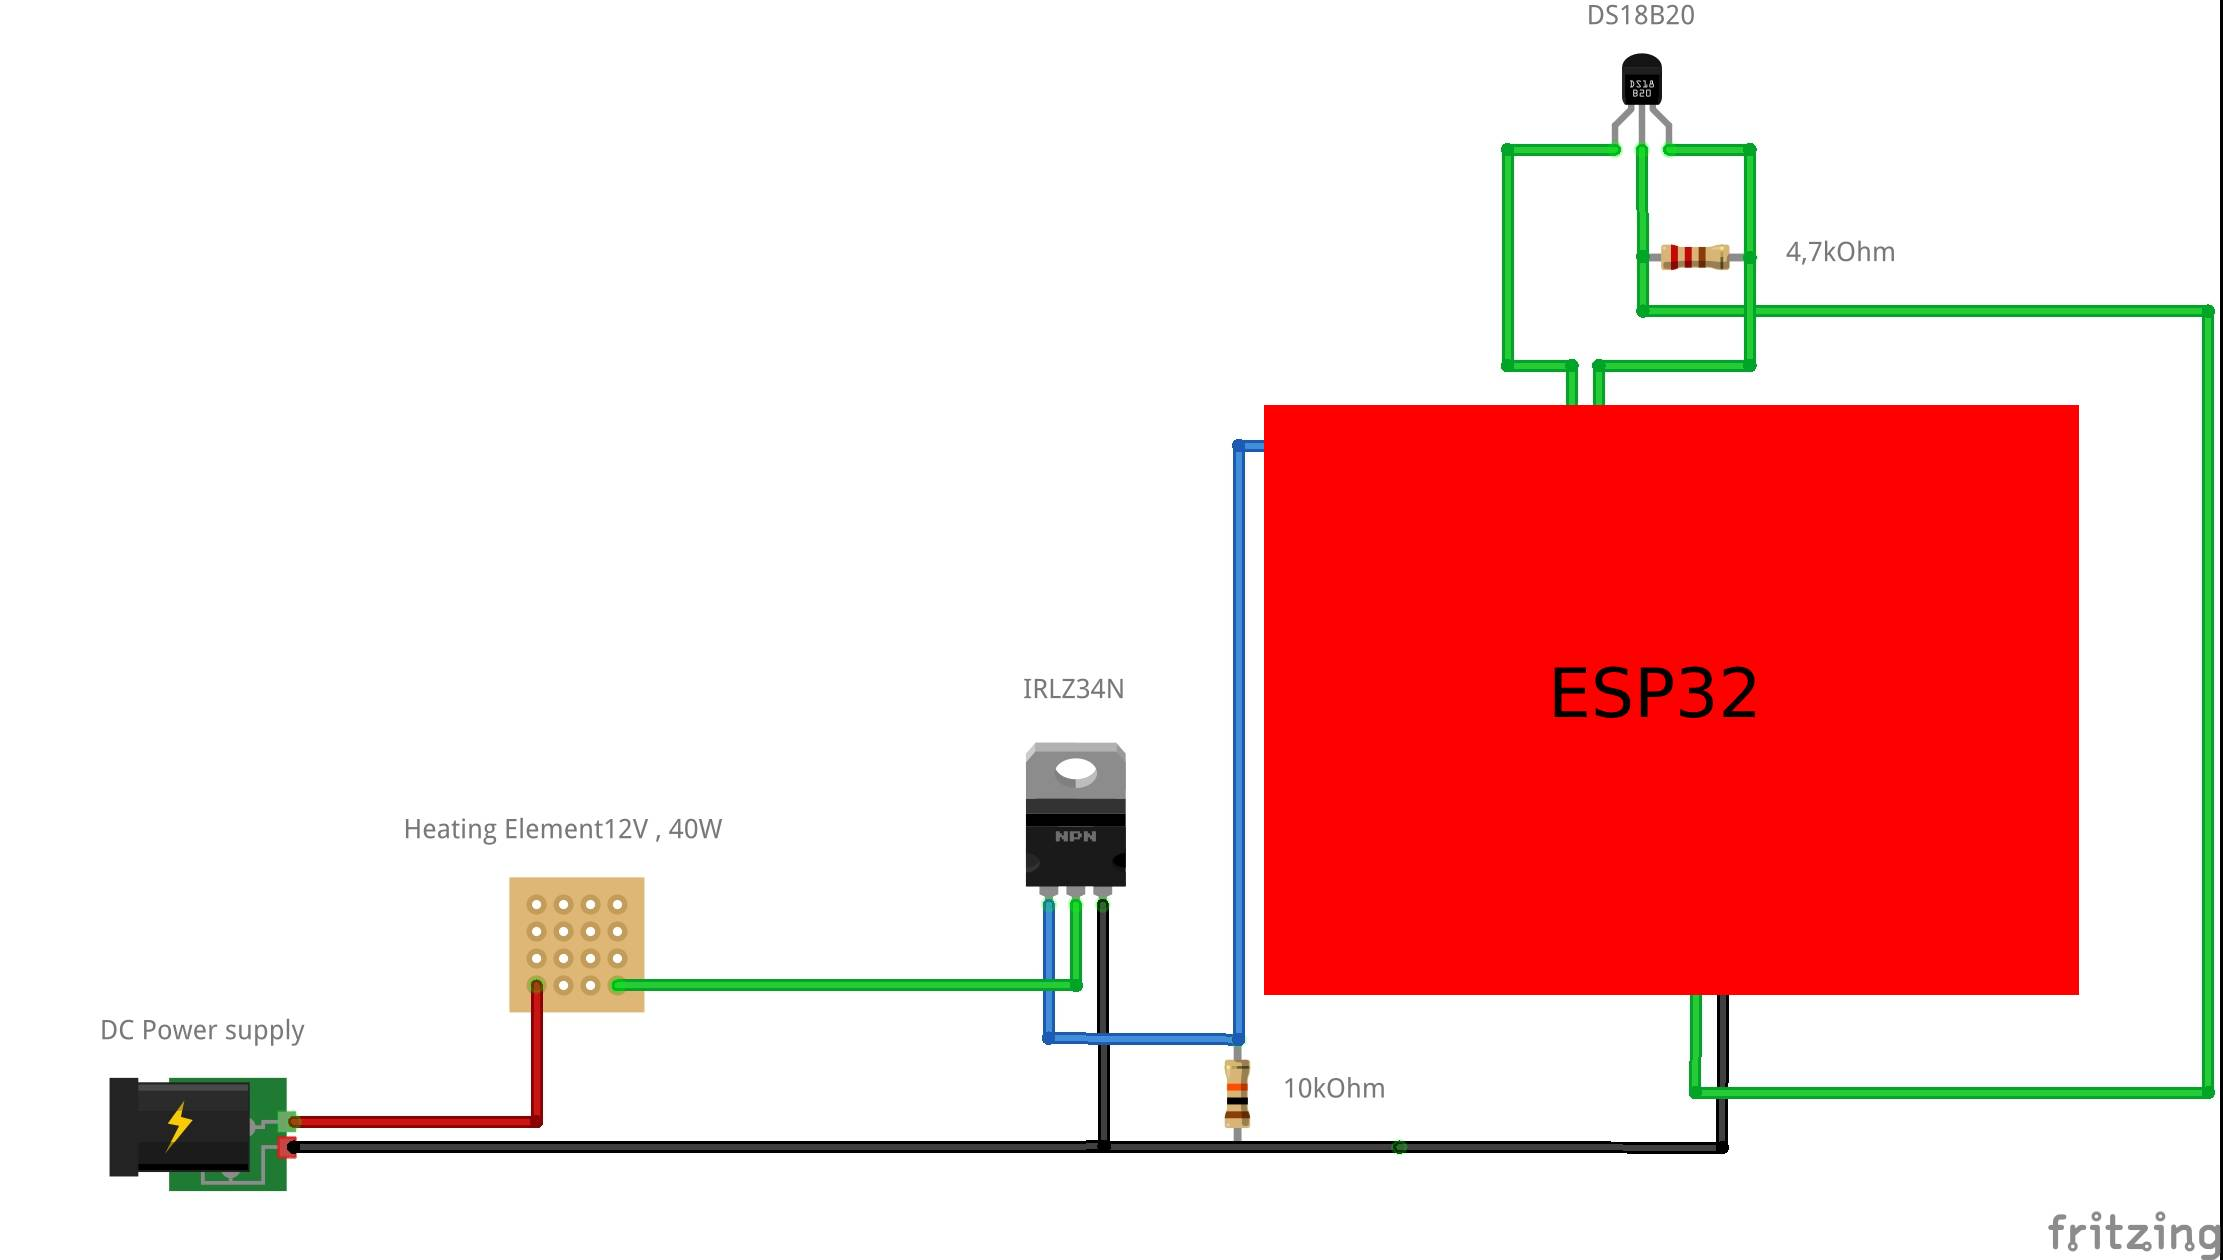
\includegraphics[scale=0.5]{images/temperature_control_diagram.jpg}}
	\caption{HLT Temperature Controller Diagram}
\end{figure}

\subsubsection{Source}
This requirement came from Dr. Chris Conly. He requested that our team enable
the user to be able to set a specific temperature via the main control
touchscreen. The water is to stay at a constant boiling temperature to maximize
effectiveness of the mashing process.  
\subsubsection{Standards}
\begin{itemize}
\item IEC 60730
\item IEC 60335
\item EN ISO 13849
\end{itemize}
\subsubsection{Priority}
This feature is of \textbf{Critical} priority. Without this feature we would be unable to
accomplish an effective mashing process. 

\subsection{Boiling Kettle Heating Element Temperature Management}
\subsubsection{Description}
The heating element on the boil vessel will need to maintain a water temperature of
212 degrees fahrenheit for optimal extraction. This temperature control will
managed by an ESP32 microcontroller. The temperature of the vessel will be
monitor by a DS18B20 digital thermometer. The microcontroller will take
continuous readings from the thermometer. When it begins dropping below the
desire temperature the microcontroller will send a signal to a mosfet. When the
mosfet receives that signal it switch states and allow for power to be delivered
to the heating element. Once the desired temperature is reached, the
microcontroller will send another signal to the mosfet. The mosfet will then
turn off, and this would turn off the power to the heating element.

\begin{figure}[H]
	\centering
	\graphicspath{.\images}
	\fbox{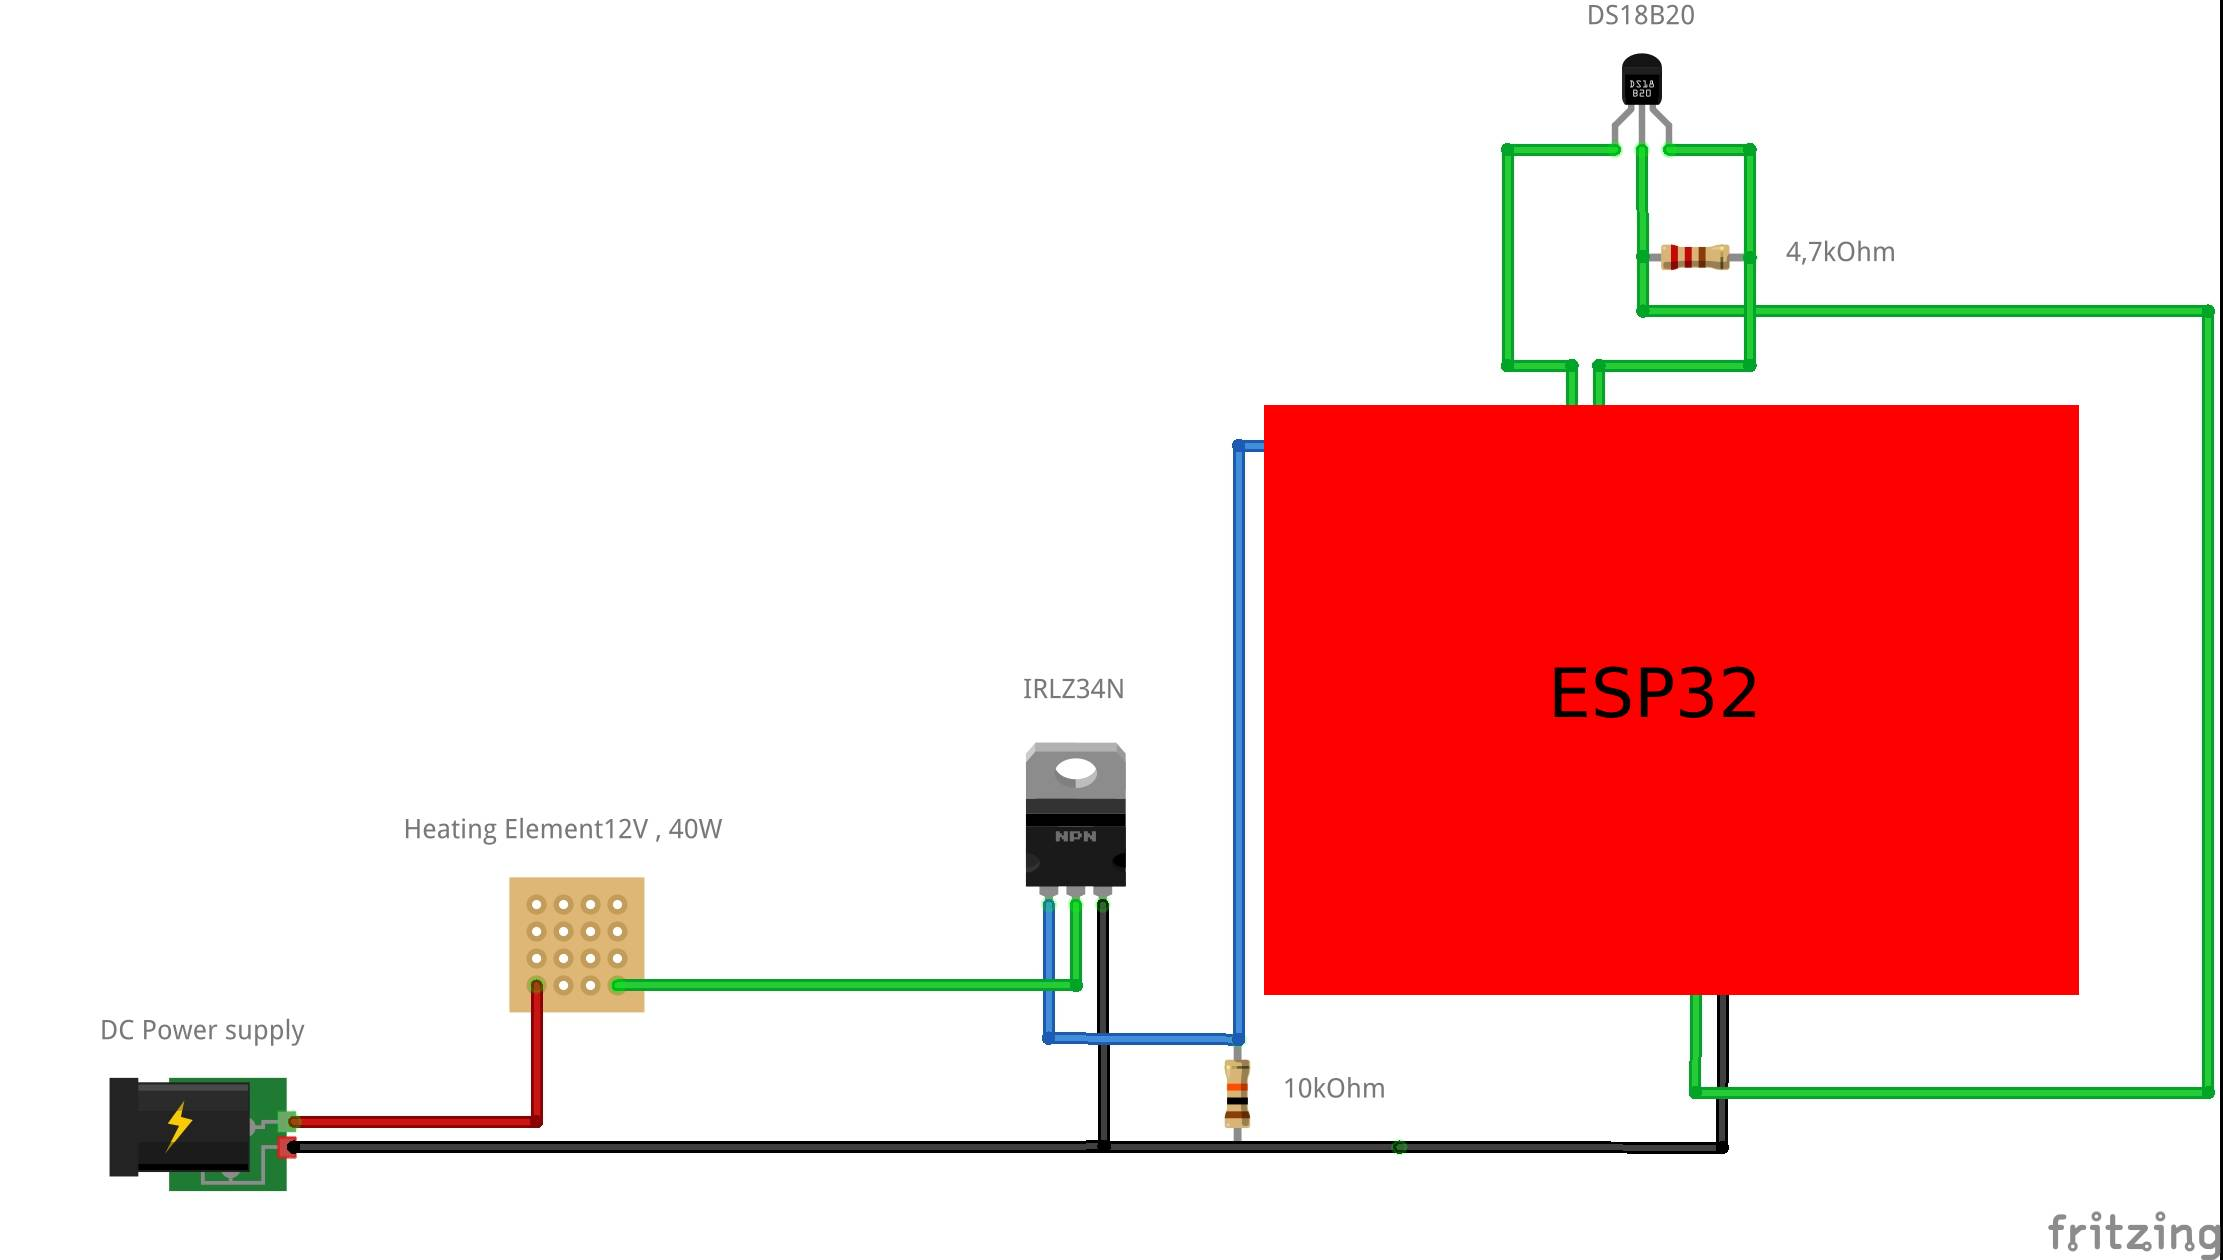
\includegraphics[scale=0.5]{images/temperature_control_diagram.jpg}}
	\caption{Boiling Kettle Temperature Controller Diagram}
\end{figure}

\subsubsection{Source}
This requirement came from Dr. Chris Conly. He requested that our team ensure
that the water stay a constant boiling temperature to maximize extraction.  
\subsubsection{Constraints}
Detailed description of applicable constraints...
\subsubsection{Standards}
\begin{itemize}
\item IEC 60730
\item IEC 60335
\item EN ISO 13849
\end{itemize}
\subsubsection{Priority}
This feature is of \textbf{Critical} priority. Without this feature we would be unable to
accomplish any sort of extraction. 

\newpage
\section{Packaging Requirements}
The system will be packaged as a set of components that can be attached to any four kettle brewing system. As most customers will have some sort of four kettle brewing system that can simple be modified. All software will be pre-installed onto all electrical hardware.

\subsection{Modular part storage}
\subsubsection{Description}
All of the device will packaged and shipped as a set of components that can be added onto a four kettle brewing system. Packaging will include instructions for hardware installation and setup. Software will be pre-installed in all locations applicable.
\subsubsection{Constraints}
Water tight packaging is required to protect electrical equipment. 
\subsubsection{Standards}
Not applicable
\subsubsection{Priority}
This should be given low priority.

\newpage
\section{Performance Requirements}
Include a header paragraph specific to your product here. Performance requirements address items such as: how fast specific critical operations must complete; how long it takes to start/stop activities; how long the battery must last; maximum time it must take to set up; etc.

\subsection{Requirement Name}
\subsubsection{Description}
Detailed requirement description...
\subsubsection{Source}
Source
\subsubsection{Constraints}
Detailed description of applicable constraints...
\subsubsection{Standards}
List of applicable standards
\subsubsection{Priority}
Priority
\newpage
\section{Safety Requirements}
Include a header paragraph specific to your product here. Safety requirements might address items specific to your product such as: no exposure to toxic chemicals; lack of sharp edges that could harm a user; no breakable glass in the enclosure; no direct eye exposure to infrared/laser beams; packaging/grounding of electrical connections to avoid shock; etc.

This section will provide brief explanation on safety requirement while using this product. There are various risk factors included while operating the Brewing system. Since we are dealing with electrical appliances, there is always a risk of getting electrocuted if proper attention is not given. 

\subsection{Safety Hazards while Working with the Electricity}
\subsubsection{Description}
Different electrical appliances like electric heater will be used in this project alongside with water. Even a small misplaced or leakage of water into the micro controller can damage it and can put the user in electrical hazards. While working with mash, it is important to note how hot the mash is in order to prevent burn.

\subsubsection{Source}
A basic safety measure taken while working with any electrical appliances, especially when a liquid is nearby.

\subsubsection{Constraints}
The product must be built closed to a place where there is electrical plugs. Once built, the product can be difficult and time-consuming to move. The user should be present at the site while brewing at first for some batches to make sure everything is running smoothly.

\subsubsection{Standards}
Non-applicable.

\subsubsection{Priority}
Top-priority should be given as this is concerned with the health of the user.
\newpage
\section{Maintenance \& Support Requirements}
Include a header paragraph specific to your product here. Maintenance and support requirements address items specific to the ongoing maintenance and support of your product after delivery. Think of these requirements as if you were the ones who would be responsible for caring for customers/end user after the product is delivered in its final form and in use "in the field". What would you require to do this job? Specify items such as: where, how and who must be able to maintain the product to correct errors, hardware failures, etc.; required support/troubleshooting manuals/guides; availability/documentation of source code; related technical documentation that must be available for maintainers; specific/unique tools required for maintenance; specific software/environment required for maintenance; etc.

\subsection{Digital User Manual}
\subsubsection{Description}
The web app will have a digital copy of the user manual available, which the user can download at any time.
\subsubsection{Source}
Marcos Juarez
\subsubsection{Constraints}
The server would have to be up at all times to respond to the download request
\subsubsection{Standards}
N/A
\subsubsection{Priority}
High

\subsection{Bug Reporting}
\subsubsection{Description}
The web app will have a way of reporting bugs to the server so the team can address them.
\subsubsection{Source}
Marcos Juarez
\subsubsection{Constraints}
The server would have to always listen for these reports
\subsubsection{Standards}
N/A
\subsubsection{Priority}
Moderate

\subsection{Contact us section}
\subsubsection{Description}
A section on the web app with a way to contact the team will be available to the user for technical issues and/or support
\subsubsection{Source}
Marcos Juarez
\subsubsection{Constraints}
The team would have to regularly check the email or wherever the customer message is sent.
\subsubsection{Standards}
N/A
\subsubsection{Priority}
Low
\newpage
\section{Other Requirements}
Include a header paragraph specific to your product here. In this section specify anything else that is required for the product to be deemed complete. Include requirements related to customer setup and configuration if not specified in a previous requirement. Add any known requirements related to product architecture/design, such as modularity, extensibility (for future enhancements), or adaptation for a specific programming language. Consider requirements such as portability of your source code to various platforms (Windows, Linux, Unix Mac OS, etc.).

\subsection{Requirement Name}
\subsubsection{Description}
Detailed requirement description...
\subsubsection{Source}
Source
\subsubsection{Constraints}
Detailed description of applicable constraints...
\subsubsection{Standards}
List of applicable standards
\subsubsection{Priority}
Priority
\newpage
\section{Future Items}
In this last section, you will reiterate all requirements that are listed as priority 5. This is repetitive, but necessary as a concise statement of features/functions that were considered/discussed and documented herein, but will NOT be addressed in the prototype version of the product due to constraints of budget, time, skills, technology, feasibility analysis, etc. Use the following format for this section.

\subsection{Requirement Name}
\subsubsection{Description}
Detailed requirement description...
\subsubsection{Source}
Source
\subsubsection{Constraints}
Detailed description of applicable constraints...
\subsubsection{Standards}
List of applicable standards
\subsubsection{Priority}
Priority
\newpage

%%% References
\bibliographystyle{plain}
\bibliographystyle{reference/IEEEtran_custom}
\bibliography{reference/refs}{}

\end{document}